\chapter{Introducción específica} % Main chapter title

\label{Chapter2}

%----------------------------------------------------------------------------------------
%	SECTION 1
%----------------------------------------------------------------------------------------
En el presente capítulo se describen los componentes de hardware, software y herramientas utilizados para realizar el trabajo.

\section{Estructura del sistema}

En las siguientes secciones se describe la estructura del sistema, con un enfoque en los sistemas embebidos, la detección de objetos y el prototipo KiwiScan.

\subsection{Los sistemas embebidos}

En el contexto de la agricultura moderna están diseñados para realizar tareas específicas y en tiempo real. En el caso de KiwiScan para la plantación de kiwi, el sistema se compone de una serie de módulos, como cámaras, sensores, pantallas y unidades de almacenamiento. Este podrá montarse en un medio de transporte adecuado a las características de la plantación, lo que permite la captura automatizada de imágenes de los frutos, así como el registro de datos ambientales relevantes durante el recorrido. Los datos recolectados se almacenan localmente en una tarjeta microSD.

\subsection{Detección de Objetos}

La detección de objetos es una técnica avanzada de visión por computadora que permite identificar y clasificar objetos en las imágenes. Esta tecnología, ha demostrado ser particularmente valiosa en el ámbito agrícola, donde la precisión en la estimación de la producción y la gestión eficiente de recursos son esenciales \citep{Lim2020}. 

Para que la detección de objetos funcione correctamente, se requiere de un conjunto de imágenes de entrada. Luego, estas son procesadas mediante algoritmos de visión por computadora. Estos algoritmos analizan las imágenes para identificar y contar los frutos \citep{Montiel2019}.

La detección de objetos se basa en técnicas avanzadas, como el análisis de imágenes y el aprendizaje automático, que permiten distinguir entre kiwis maduros, inmaduros y otros objetos presentes en la plantación.

\newpage

\subsection{El prototipo KiwiScan}

El prototipo desarrollado, a partir de ahora denominado KiwiScan, está conformado por tres partes esenciales que permiten llevar a cabo su labor. Estas son:
\begin{itemize}
\item El nodo sensor: esta es la parte física o hardware del sistema, utilizado para adquirir las imágenes de la plantación.
\item El firmware: este abarca la lógica del sistema y se encarga de la adquisición, procesamiento y la gestión del almacenamiento de datos. Puede funcionar sobre un sistema operativo de tiempo real o no.
\item El modelo de detección de objetos: este permite realizar la contabilización de los frutos encontrados en las imágenes proporcionadas como entrada.
\end{itemize}

\section{Componentes principales de hardware}

En esta sección se describen en detalle los componentes de hardware seleccionados para este trabajo, que resultaron clave para garantizar el funcionamiento adecuado del prototipo.

\subsection{Plataforma de desarrollo STM32 Nucleo-F429ZI}
\label{subsec:F429ZI}

La placa STM32 Nucleo-F429ZI, que se muestra en la figura \ref{fig:STM32-F429ZI}, posee un núcleo ARM Cortex-M4. Esta placa ofrece una plataforma flexible para desarrollar aplicaciones embebidas, con una amplia variedad de interfaces y periféricos, como ADC, DAC, GPIO, SPI, I2C, USART, entre otros. Además, cuenta con compatibilidad con los ecosistemas Arduino y ST Morpho, lo que facilita la expansión y el prototipado rápido. Es ideal para proyectos que requieren procesamiento en tiempo real, gestión de múltiples tareas y alto rendimiento \citep{WEBSITE:Itt2024}.

Características:
\begin{itemize}
\item STM32F429ZIT6 en paquete LQFP144.
\item CPU ARM® Cortex®-M4 de 32 bits con FPU.
\item Frecuencia máxima de CPU de 180 MHz.
\item VDD de 1,8 V a 3,6 V.
\item Flash de 2048 KB.
\item GPIO (114) con capacidad de interrupción externa.
\item Controlador DMA de 16 flujos con FIFO y compatibilidad con ráfagas.
\item Temporizador de control avanzado.
\item Temporizadores de uso general.
\item CAN 2.0B activo.
\item USB 2.0 OTG SA.
\item I2C.
\item SPI.
\item USART/UART.
\item EFS.
\item SDIO.
\item Generador aleatorio (TRNG para entropía HW).
\item Ethernet.
\end{itemize}

\begin{figure}[htbp]
	\centering
	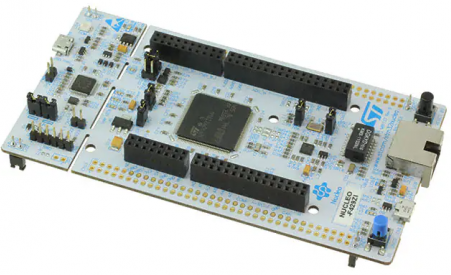
\includegraphics[width=.5\textwidth]{./Figures/STM32-F429ZI.png}
	\caption{Plataforma de desarrollo Nucleo-F429ZI\protect\footnotemark.}
	\label{fig:STM32-F429ZI}
\end{figure}

\footnotetext{Imagen tomada de \url{https://tienda.ityt.com.ar/plataforma-stm32/12702-nucleo-f429zi-stm32f429zi-stm32-cortex-m4-arm-itytarg.html}}

\subsection{Sensor de temperatura y humedad DHT11}
\label{subsec:dht11}

Este dispositivo, presentado en la figura \ref{fig:Dht11}, se utiliza para medir temperatura y humedad en ambientes controlados. Es altamente popular debido a su bajo costo y facilidad de uso. Dispone de un sensor capacitivo para medir la humedad y un termistor para la temperatura. El DHT11 proporciona lecturas de humedad en un rango del 20\% al 90\% con una precisión de ±5\%, y de temperatura entre 0 °C y 50 °C con una precisión de ±2 °C. Se comunica mediante una señal digital, lo que lo hace ideal para aplicaciones en sistemas embebidos y proyectos medianos \citep{WEBSITE:Dht112024}.

\begin{figure}[htbp]
	\centering
	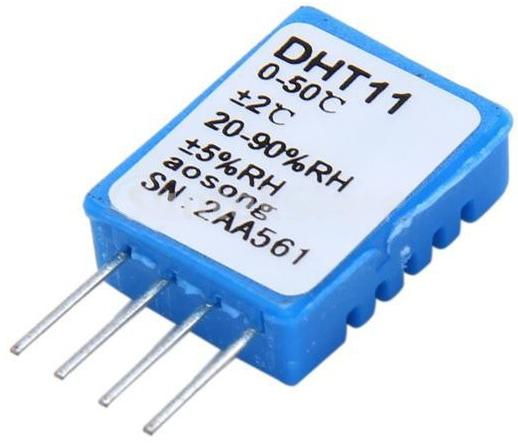
\includegraphics[width=.5\textwidth]{./Figures/dht11.png}
	\caption{Sensor de temperatura y humedad DHT11\protect\footnotemark.}
	\label{fig:Dht11}
\end{figure}

\footnotetext{Imagen tomada de \url{https://www.todomicro.com.ar/sensores/224-sensor-de-temperatura-y-humedad-dht11-arduino.html}}

\newpage

\subsection{Display LCD}
\label{subsec:DisplayLCD}

Esta pantalla, capaz de mostrar hasta 16 caracteres en 2 filas, se presenta en la figura \citep{WEBSITE:lcd2024}. Se utiliza en proyectos de electrónica y sistemas embebidos debido a su simplicidad y bajo costo. Cada carácter se forma a partir de una matriz de puntos de 5 x 8 píxeles, lo que permite visualizar letras, números y símbolos. El display es compatible con microcontroladores y microprocesadores, y se controla mediante interfaces paralelas o serie. Resulta ideal para mostrar información básica, como datos de sensores, mensajes o indicadores de estado en tiempo real \citep{WEBSITE:lcd2024}.

\begin{figure}[htbp]
	\centering
	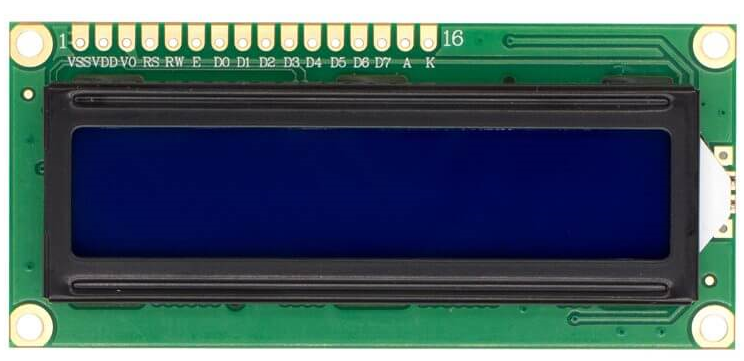
\includegraphics[width=.5\textwidth]{./Figures/lcd.png}
	\caption{Display LCD\protect\footnotemark.}
	\label{fig:lcd2024}
\end{figure}

\footnotetext{Imagen tomada de \url{https://uelectronics.com/producto/display-lcd-16x2-fondo-azul-amarillo/?srsltid=AfmBOorkJNNBhdEHSHGVr8xleeZYs_HXpCKmLdXyXVL5B2i6Fe4fKk0r}}

\subsection{Cámara Ov7670}
\label{subsec:camara}

Este módulo compacto de captura de imágenes, mostrado en la figura \ref{fig:camara2024}, se utiliza en proyectos de visión por computadora y sistemas embebidos. El sensor de imagen CMOS Ov7670 puede capturar imágenes en resolución VGA (640x480) y CIF (352x288), lo que lo hace adecuado para aplicaciones de procesamiento de imágenes, seguimiento de objetos y reconocimiento de patrones. La cámara se conecta a microcontroladores o plataformas de desarrollo como Arduino y STM32 mediante interfaces I2C o SCCB para configuración, y una interfaz de datos paralela para la transferencia de imágenes. Además, el módulo ofrece control automático de exposición, balance de blancos y eliminación de ruido, lo que garantiza imágenes de calidad en diversas condiciones de luz \citep{WEBSITE:camara2024}.

\begin{figure}[htbp]
	\centering
	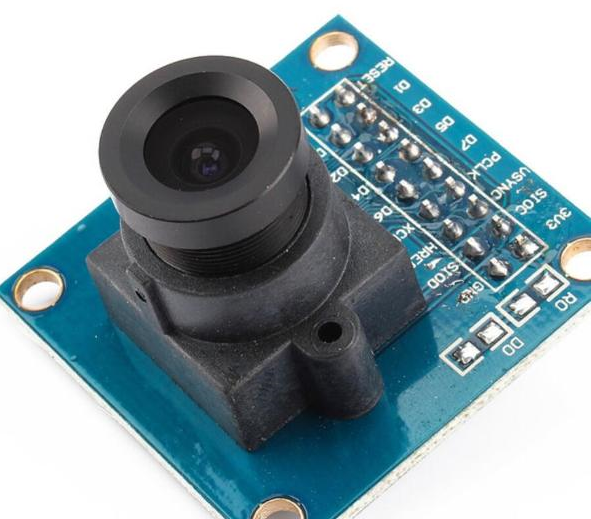
\includegraphics[width=.5\textwidth]{./Figures/camara.png}
	\caption{Cámara Ov7670\protect\footnotemark.}
	\label{fig:camara2024}
\end{figure}

\footnotetext{Imagen tomada de \url{https://www.arcaelectronica.com/products/modulo-de-camara-ov7670-arduino?srsltid=AfmBOopgmnm_0gtPYtNMaSrCGCOKnXMwbjdXpUfh84WJ_Hi9V3akPCPp}}

\subsection{Sensor ultrasónico HC-SR04}
\label{subsec:hcsr04}

Este dispositivo, mostrado en la figura \ref{fig:hcsr2024}, se utiliza para medir distancias con precisión en proyectos de robótica, sistemas embebidos y automatización. Emite ondas ultrasónicas que se reflejan en objetos cercanos y luego las capta el sensor. El tiempo que tarda la señal en regresar permite calcular la distancia al objeto. El HC-SR04 ofrece un rango de medición de 2 cm a 4 m, con una precisión de aproximadamente 3 mm. Se integra fácilmente con microcontroladores como Arduino o STM32 mediante un sistema de disparo y recepción de señal. Es ideal para aplicaciones como evitar obstáculos, medir niveles de líquido y sistemas de detección de proximidad \citep{WEBSITE:hcsr2024}.

\begin{figure}[htbp]
	\centering
	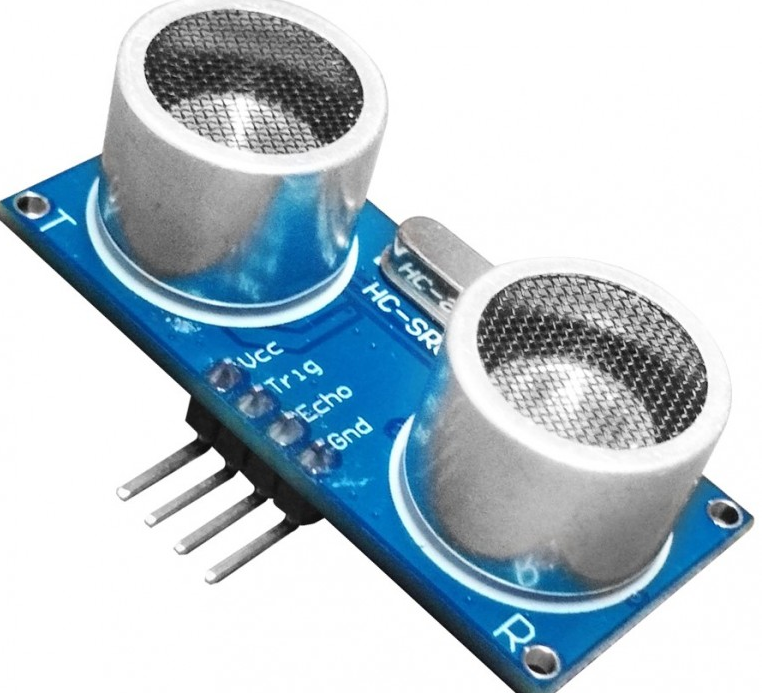
\includegraphics[width=.5\textwidth]{./Figures/hcsr04.png}
	\caption{Sensor ultrasónico HC-SR04\protect\footnotemark.}
	\label{fig:hcsr2024}
\end{figure}

\footnotetext{Imagen tomada de \url{https://www.todomicro.com.ar/modulos/81-sensor-ultrasonico-ultrasonido-hc-sr04-arduino-pic-robotica.html}}

\section{Herramientas de software y testing utilizados}

Las herramientas de software seleccionadas para este trabajo fueron fundamentales para el desarrollo y las pruebas del prototipo. A continuación se describen en detalle las características principales y los casos de uso de cada una.

\subsection{STM32 CubeIDE}
\label{subsec:stm32}

El sistema STM32 CubeIDE es un entorno de desarrollo integrado (IDE) creado por STMicroelectronics para trabajar con microcontroladores STM32. Basado en Eclipse, STM32 CubeIDE permite a los desarrolladores escribir, compilar y depurar código en lenguajes como C y C++ y por lo tanto facilita el desarrollo de aplicaciones embebidas. También integra herramientas como STM32CubeMX, que configura los periféricos del microcontrolador y genera código automáticamente. Estas  características contribuyen a reducir los errores y a acelerar el proceso de desarrollo. STM32 CubeIDE es compatible con sistemas operativos como Windows, macOS y Linux, y soporta una amplia gama de microcontroladores de la familia STM32, lo que lo convierte en una opción flexible para proyectos de sistemas embebidos \citep{WEBSITE:stm32}.

\subsection{Sistema operativo FreeRTOS}
\label{subsec:FreeRTOS}

Es un sistema operativo en tiempo real (RTOS) de código abierto, ampliamente utilizado en el desarrollo de aplicaciones embebidas. Diseñado para microcontroladores y sistemas de baja potencia, FreeRTOS ofrece un \textit{kernel} ligero y eficiente para gestionar tareas concurrentes de manera óptima. Soporta características clave como multitarea, gestión de memoria, sincronización entre tareas y temporización precisa, lo que lo convierte en una solución ideal para aplicaciones que requieren control preciso del tiempo y recursos limitados.

Además, FreeRTOS es compatible con una amplia variedad de arquitecturas de microcontroladores, incluidos los STM32. Cuenta con una extensa comunidad y soporte comercial a través de \textit{partners} como Amazon Web Services (AWS), que ofrece una versión ampliada llamada FreeRTOS IoT. Gracias a su escalabilidad y flexibilidad, FreeRTOS es una opción popular en proyectos que van desde dispositivos portátiles hasta sistemas industriales complejos \citep{WEBSITE:freertos}.

\subsection{Pruebas en CEEDLING}
\label{subsec:CEEDLING}

Es una herramienta de testing para proyectos en lenguaje C, diseñada para facilitar el desarrollo y la prueba de software embebido. Este marco de pruebas automatizado proporciona un entorno completo para la creación, ejecución y gestión de pruebas unitarias.

Ceedling integra varias herramientas esenciales para el testing, como CMock, un generador de mocks que simula dependencias y facilita el aislamiento de unidades de código durante las pruebas. Además, utiliza Unity, un framework de pruebas unitarias para C, que ofrece una serie de aserciones y macros para verificar el comportamiento del código.

La configuración y ejecución de pruebas con Ceedling se realizan a través de un archivo de configuración, lo que permite una integración fluida en el proceso de desarrollo. La herramienta soporta la ejecución de pruebas en diferentes entornos, genera informes detallados de cobertura de código y facilita la identificación de errores y defectos en el software \citep{WEBSITE:CEEDLING}.

\section{Protocolos de comunicación}

Los protocolos de comunicación seleccionados son esenciales para la interacción entre los diferentes componentes del sistema. UART permite la transmisión y recepción de datos de manera eficiente, lo que facilita la conexión entre microcontroladores y dispositivos periféricos.

I2C, por otra parte, ofrece una solución versátil para la comunicación entre múltiples dispositivos en el sistema. Su capacidad para identificar dispositivos mediante direcciones únicas garantiza una integración efectiva de sensores y otros periféricos, y de esta manera contribuye a optimizar la funcionalidad del prototipo.

\subsection{El protocolo UART}
\label{subsec:UART}

Es un protocolo de comunicación serial utilizado en sistemas embebidos y en la comunicación entre dispositivos electrónicos. UART permite la transmisión y recepción de datos en serie, es decir, un bit a la vez, a través de un solo canal de comunicación.

El funcionamiento de UART se basa en una comunicación asíncrona, lo que significa que no requiere una señal de reloj compartida entre los dispositivos que se comunican. En su lugar, utiliza parámetros de configuración como la velocidad de transmisión (\textit{baud rate}), la paridad, el número de bits de datos y el número de bits de parada para sincronizar la transmisión y recepción de datos. En la práctica, UART se emplea para conectar microcontroladores, módulos de comunicación, sensores y otros dispositivos electrónicos, lo que facilita la transferencia de datos \citep{WEBSITE:uart}. 

\subsection{El protocolo I2C}
\label{subsec:I2C}

Es un protocolo de comunicación serial ampliamente utilizado para conectar dispositivos en sistemas embebidos. Desarrollado por Philips Semiconductors (ahora NXP), I2C facilita la comunicación entre microcontroladores, sensores, memorias y otros periféricos mediante una interfaz de dos hilos.

El protocolo I2C utiliza dos líneas para la transmisión de datos: la línea de reloj (SCL) y la línea de datos (SDA). La línea SCL sincroniza la comunicación mediante la señal de reloj, mientras que la línea SDA transporta los datos entre los dispositivos conectados. Ambos hilos son bidireccionales, lo que permite que tanto el maestro como el esclavo envíen y reciban información.

I2C permite la comunicación en un bus que puede conectar múltiples dispositivos mediante una sola pareja de líneas. Cada dispositivo en el bus I2C tiene una dirección única que permite su identificación. Su implementación en sistemas embebidos abarca aplicaciones como la comunicación con sensores, controladores de pantallas y dispositivos de almacenamiento \citep{WEBSITE:i2c}.
